
Um motor DC é essencialmente uma máquina elétrica de corrente contínua, que
converte energia elétrica de corrente contínua em energia mecânica. Máquinas
elétricas de corrente contínua são mais fácies de se controlar (quando
comparadas a máquinas de corrente alternada) e oferecem uma grande faixa de
velocidades \cite{Maquinas_eletricas}. Devido a essas características, tornam-se
boas candidatas para uso em eletrônica e robótica, uma vez que é viável
utilizá-las com com baterias. Para controlar a velocidade de um motor, é
necessário o uso de um encoder, que converte o sinal de posição em um valor
mensurável de velocidade angular, e também um driver, que permite a
microcontroladores controlarem a atuação do motor.

\subsection{Encoder magnético}

	Encoders magnéticos são um tipo de encoder rotacional que utiliza sensores 
	para identificar alterações em campos magnéticos a partir de uma roda ou 
	anel magnéticos. A rotação detectada é expressa em termos de pulsos de maior
	ou menor duração, a depender da resolução do encoder. Um encoder incremental
	mede a posição relativa do eixo (em contraste com encoders absolutos), em
	incrementos, a partir de dois sensores magnéticos, indicando a quantidade de
	pulsos percorridos entre a posição de referência e a posição atual.
	
	Há alguns tipos diferentes de se medir e representar a resolução de um
	encoder magnético. Na representação de pulsos por revolução (PPR), o valor 
	apresentado descreve o número de pulsos em valor alto que um encoder terá em
	qualquer uma das suas duas saídas quadráticas. Uma outra representação comum
	de resolução de encoders é CPR (contagens por revolução), que representa o
	número de estados de quadratura decodificados que existem entre as duas
	saídas do encoder (representando, portanto, o valor de uma resolução dada em
	PPR multiplicada por 4). Outras formas de representar a resolução de um
	encoder são LPR (linhas por revolução, referindo-se a às barras marcadas no
	disco óptico de um encoder, cada uma representando um pulso de valor baixo),
	e também ciclos por revolução (cujo acrônimo ocasionalmente é dado também
	como CPR por fabricantes) - o valor apresentado em ambas as representações 
	equivale à representação em PPR (que é a representação adotada para
	avaliação e apresentação dos componentes utilizados neste trabalho). 
	
	Em encoders magnéticos incrementais, são produzidas duas ondas quadradas
	como saídas, A e B \cite{encoder_ppr}. As duas possuem 90° de fase entre si,
	e, caso a onda A esteja adiantada em relação a B (\ref{encoder_ppr_ab}),
	o sentido de rotação é positivo (anti-horário).

\begin{figure}[h]
	\centering
	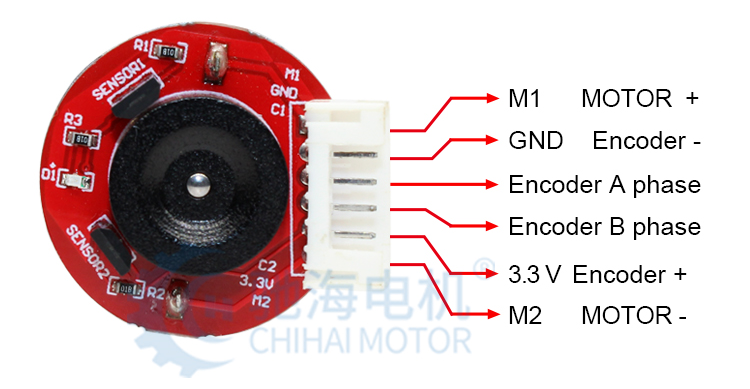
\includegraphics[width=0.6\textwidth]{figures/encoder_holzer}
	\caption{Encoder holzer \cite{motor_dc_6v_encoder}}
\end{figure}

\begin{figure}[h]
	\centering
	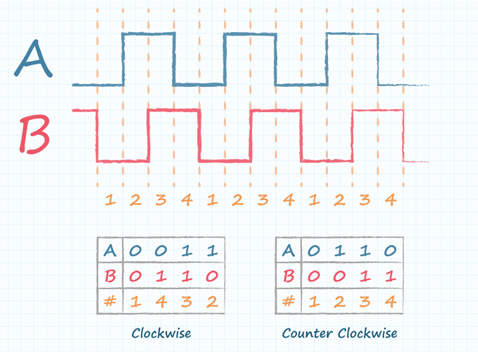
\includegraphics[width=0.6\textwidth]{figures/encoder_pulso_ab}
	\caption{Ondas quadradas resultantes dos pulsos de saída do encoder \cite{encoder_ppr}}
	\label{encoder_ppr_ab}
\end{figure}


\subsection{Driver para motor}

	Motores não podem ser ligados diretamente nos pinos de um microcontrolador -
	é necessário um circuito que permita à baixa corrente do microcontrolador
	controlar correntes mais altas, como as de um motor DC. Drivers podem ser
	usados em uma variedade de tensões de entrada e permitem o controle da
	velocidade por PWM \cite{toshiba_ponte_h}.

	O driver a ser usado neste trabalho é do tipo ponte H. A Ponte H permite que
	a polaridade da alimentação do motor DC seja alterada. Devido a sua inércia,
	o motor continua girando mesmo quando a energia é retirada, mas a ponte H
	pode curto-circuitar seus terminais, gerando uma força eletromotriz de
	frenagem. Outra razão para uso de um driver ponte é a necessidade de se lidar
	com a tensão gerada pelo motor quando o rotor continua a girar após remover
	alimentação - o motor se comporta com um gerador nesse momento, e a ponte H
	fornece um caminho livre para essa corrente gerada.


